\documentclass[../main.tex]{subfiles}
\graphicspath{{\subfix{../figures/}}}

\begin{document}
    Diese Arbeit beschäftigt sich mit der epidemiologischen Modellierung des weiteren Verlaufs von Covid-19. Um vertretbare Annahmen treffen zu können, muss das Anwendungsproblem zunächst genauer betrachtet werden.

    Covid-19 wird durch das Corona-Virus SARS-CoV-2 ausgelöst. Eine Infektion ist medizinisch nachweisbar, sodass umfangreiches Testen eine Einschätzung der Lage ermöglichen kann.
    
    Es werden mehrere Datensätze verwendet, welche nachgewiesene Neuinfektionen (vgl. \cite{Hei22}), Impfungen (vgl. \cite{BMG22}) und Intensivbelegung (vgl. \cite{DIVI22}) im Zusammenhang mit Covid-19 erfassen\footnote{Informationen zur Auswertung der Datensätze im Anhang (S. \pageref{ap:evaluation})}.

    Seit dem erstmaligen Auftreten von Covid-19 in Deutschland zu Beginn des Jahres 2020 sind mehrere Infektionswellen aufgetreten, die ihren Höhepunkt meist im Winterhalbjahr erreichten und in Abbildung \ref{fig:covid19_incidence} dargestellt sind.

    \begin{figure}[b]
        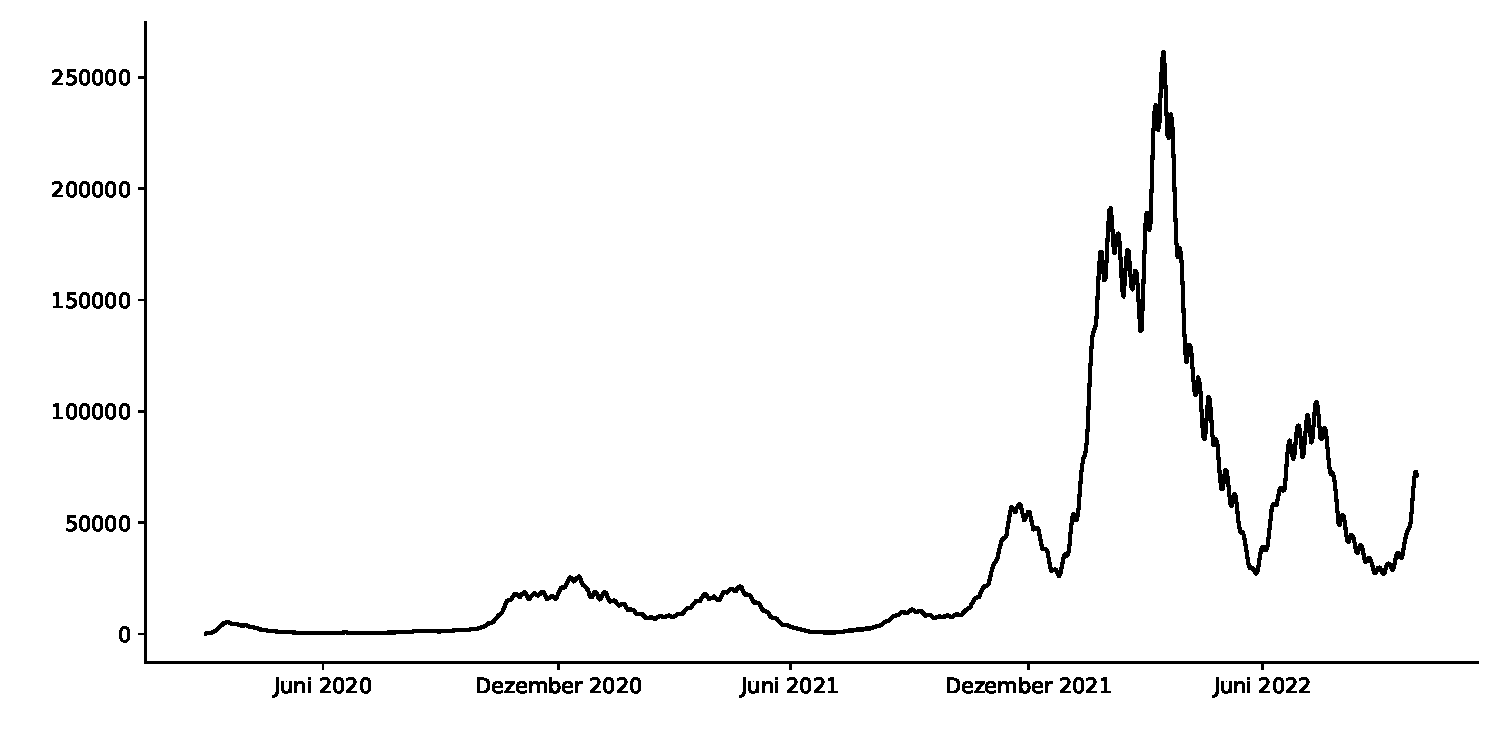
\includegraphics[width=0.9\textwidth]{incidence.pdf}
        \caption{Tägliche Covid-19-Neuinfektionen in Deutschland}
        \label{fig:covid19_incidence}
    \end{figure}

    \subsection{Epidemiologische Aspekte}
    \label{ssec:epidemiological_aspects}
    Covid-19 wird mittels kleiner Partikel über die Atemwege übertragen (vgl. \cite[Übertragungswege]{RKI21}). Seit Beginn der Pandemie sind neue Varianten entstanden, wobei aktuell die Omikron-Sublinie BA.5 vorherrscht (vgl. \cite[Omikron (B.1.1.529)]{RKI22}). Dabei hat sich die Kontagiosität des Virus erhöht, sodass die Basisreproduktionszahl der Omikron-Variante auf $9.5$ geschätzt wird (vgl. \cite[S. 4]{RL22}). Die Schwere der Erkrankung hat sich dabei abgemildert (vgl. \cite[Klinische Manifestation und Krankheitsschwere]{RKI22}).

    Infizierte entwickeln vielfältige Symptome, die in ihrer Schwere stark variieren. Die Erkrankung kann sich als Fieber, Husten, Geruchs- und Geschmacksverlust äußern und bis zum Lungenversagen führen; gleichzeitig treten asymptomatische Verläufe auf (vgl. \cite[Demographische Faktoren, Symptome und Krankheitsverlauf]{RKI21}).
    Die Ansteckungsfähigkeit ist kurz vor Symptombeginn am höchsten, was eine rechtzeitige Isolierung erschwert und geht nach zehn Tagen deutlich zurück (vgl. \cite[Dauer der Ansteckungsfähigkeit]{RKI21}).

    Des Weiteren führen saisonale Einflüsse auf der Nordhalbkugel zu Schwankungen der Übertragbarkeit um etwa $46\%$ (vgl. \cite[S. 1]{Liu+21}).

    Eine Infektion mit Covid-19 verleiht Immunität, welche sich nach aktuellem Wissensstand am Antikörpertiter bemisst. Der Einfluss der B- und T-Zellen, welche in Verbindung mit langanhaltender Immunität stehen, wird noch untersucht. Ein bis zwei Wochen nach der Infektion sind neutralisierende Antikörper nachweisbar, was einen Schutz vor schweren Krankheitsverläufen nahelegt, jedoch keine Reinfektion ausschließt (vgl. \cite[Immune responses and immunity to SARS-CoV-2]{ECDC22}).

    Seit Ende 2020 stehen zudem Impfstoffe zu Verfügung, die wirksam vor schweren Verläufen schützen. Der Schutz gegenüber neuen Varianten ist jedoch begrenzt und auch hier sind Durchbruchsinfektionen nicht auszuschließen (vgl. \cite[Vaccines]{ECDC22}).
    Sowohl nach Infektion als auch nach Impfung nimmt der Antikörpertiter mit der Zeit ab, was ein Verschwinden dieses Schutzes vermuten lässt (vgl. \cite[Immunität]{RKI21}). Gemäß einer Novelle des deutschen Infektionsschutzgesetzes vom 19. März 2022 gilt als immun, wer vollständig geimpft ist, das heißt eine Boosterimpfung erhalten hat, und wessen letzte durchgemachte Infektion weniger als 90 Tage zurückliegt (vgl. \cite[§22a (1,2)]{IfSG22}).

    Als Kompromiss wird daher angenommen, dass sowohl nach durchgemachter Infektion als auch nach Impfung für 90 Tage eine sogenannte sterile Immunität besteht, die vor erneuter Infektion und deren Weitergabe schützt, sowie dass dieser Immunschutz nach 90 Tagen verfällt. Durch diese Vereinfachung muss nicht zwischen mehreren Arten der Immunität unterschieden werden. 

    \subsection{Bestimmung der Ausgangssituation}
    \label{ssec:initial_state}
    Als Anfangszeitpunkt des Modells wird der 30. September 2022 gewählt. Es ist daher erforderlich, die Krankheitsverteilung in der Bevölkerung zu diesem Zeitpunkt zu kennen. Diese zählt dabei circa 83 Millionen Individuen.
    Gemäß Abschnitt \ref{ssec:epidemiological_aspects} ist infektiös ($I$), wer innerhalb der letzten zehn Tage infiziert wurde. \\Da von einer Dunkelziffer von bis zu 50\% ausgegangen werden muss, verdoppeln wir die Anzahl der in diesem Zeitraum nachgewiesenen Neuinfektionen (vgl. \cite[S. 2]{Pri+21}).
    Als immun ($R$) gilt, wessen überstandene Infektion weniger als 90 Tage zurückliegt, und wer vollständig geimpft, das heißt geboostert ist. Die übrigen Individuen sind für die Krankheit empfänglich ($S$) und es ergibt sich zum Anfangszeitpunkt folgende Verteilung:

    \begin{table}[h]
        \centering
        \begin{tabularx}{\textwidth}{X | X | X}
            \textbf{Gruppe} & \textbf{Größe} & \textbf{Anteil} \\ \hline
            $S$ & $2.6 \cdot 10^7$ & $3.13 \cdot 10^{-1}$ \\ \hline
            $I$ & $1.1 \cdot 10^6$ & $1.36 \cdot 10^{-2}$\\ \hline
            $R$ & $5.6 \cdot 10^7$ & $6.73 \cdot 10^{-1}$
        \end{tabularx}
        \caption{Gruppenverteilung zum Anfangszeitpunkt}
        \label{tab:initial_state}
    \end{table}

    Die Zahl täglich durchgeführter Impfungen gegen Covid-19 in Deutschland ist über die Woche gemittelt in Abbildung \ref{fig:vaccinations} dargestellt. Nach einem Höhepunkt im Dezember 2021 fiel diese im Sommer auf das niedrigste Niveau seit Beginn der Impfkampagne. Es kann jedoch auch in diesem Winter wieder mit einem Anstieg gerechnet werden. Daher wird angenommen, dass jeden Tag weiterhin die durchschnittliche Zahl von täglichen Impfungen zwischen erstem Januar und 30. September 2022 durchgeführt werden. Dabei handelt es sich um $117\cdot 10^3$ Impfungen, was einem Anteil von $1.4 \cdot 10^{-3}$ an der Bevölkerung entspricht.

    \begin{figure}[t]
        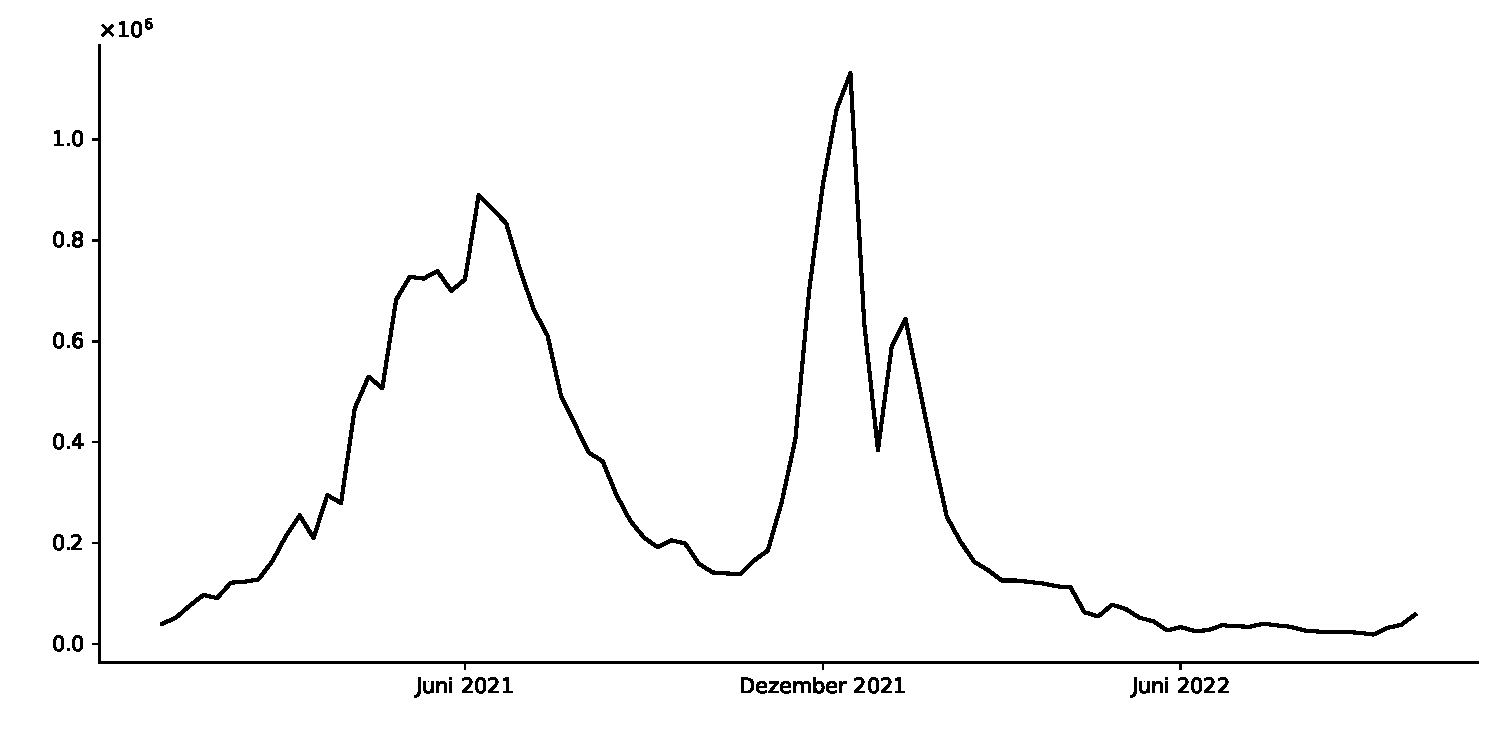
\includegraphics[width=0.9\textwidth]{vaccination.pdf}
        \caption[Tägliche Covid-19-Impfungen in Deutschland]{Tägliche Covid-19-Impfungen im Wochendurchschnitt in Deutschland}
        \label{fig:vaccinations}
    \end{figure}

    \subsection{Kapazität des Gesundheitssystems}
    \label{ssec:capacity_health_system}
    Obgleich die Krankheitsschwere der Omikron-Variante geringer ist, besteht weiterhin die Gefahr einer Überlastung, da die erhöhte Kontagiosität zu höheren Inzidenzen führt. Zur Beantwortung der Forschungsfrage muss daher zunächst definiert werden, wann von einer Überlastung des Gesundheitssystems in Deutschland gesprochen werden kann. 
    Seit Beginn der Pandemie konnte die Gesundheitsversorgung in Deutschland durchgehend sichergestellt werden. Zu den Höhepunkten der Infektionswellen kam es jedoch bereits zu Engpässen, die nicht von der Bettenkapazität, sondern vielmehr von einem Mangel an Personal ausgingen. Da der Betrieb nur durch eine hohe Belastung des Personals und die Aussetzung planbarer Eingriffe möglich war, gilt es, die Wiederholung einer solchen Situation zu vermeiden (vgl. \cite[S. 4]{Pri+21}, \cite[S. 87,89]{Cac21}).
    
    \begin{figure}[b]
        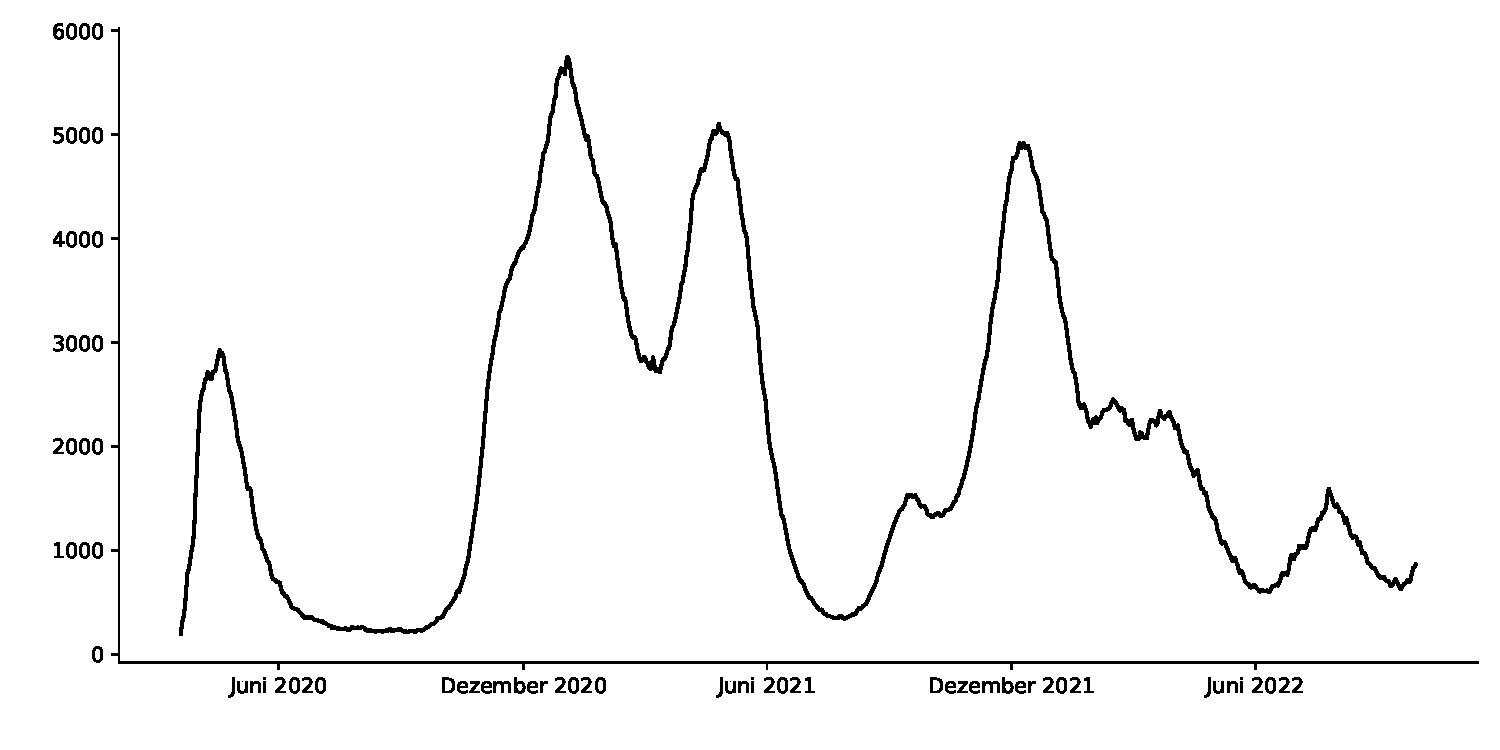
\includegraphics[width=0.9\textwidth]{icu.pdf}
        \caption{Covid-19-Patienten auf Intensivstationen in Deutschland}
        \label{fig:icu}
    \end{figure}

    Die Zahl intensivmedizinisch behandelter Covid-19-Patienten ist in Abbildung \ref{fig:icu} dargestellt und erreichte am dritten Januar 2021 mit $n = 5745$ Patienten ihren Höhepunkt. Da die Inzidenz Rückschlüsse auf die Zahl intensivpflichtiger Covid-19-Patienten erlaubt, kann ermittelt werden, wie viele Infizierte $i$ zu dieser Intensivbelastung führen (vgl. \cite[S. 3]{Pri+21}).
    Es werden ca. 0.3\% ($h_1=0.003$) der mit der Omikron-Variante Infizierten hospitalisiert (vgl. \cite[Clinical characteristics]{ECDC22}). Von allen hospitalisierten Infizierten werden wiederum 13\% ($h_2=0.13$) intensivpflichtig (vgl. \cite[S. 148]{Iul22}).
    \begin{equation*}
        i = \frac{n}{h_1 \cdot h_2} = \frac{5745}{0.003 \cdot 0.13} \approx 1.5 \cdot 10^7
    \end{equation*}
    Eine Überlastung liegt demnach ab 15 Millionen Infizierten vor.
\end{document}